
\documentclass[12pt]{article}

\usepackage{sbc-template}

\usepackage{graphicx,url}

\usepackage[brazil]{babel}   
\usepackage[utf8]{inputenc}  
\usepackage{units}
\usepackage{fancyhdr}
\pagestyle{fancy}

\fancyhead[L]{ }
\fancyhead[R]{ }

%\chead{\begin{picture}(3,3) \put(-230,-15) {\includegraphics%[width=16cm, height=2.8cm, keepaspectratio=false]{logoSIRC.png}} \end{picture}}
\renewcommand{\headrulewidth}{0pt}
\sloppy
\begin{document} 


\title{Relatório Técnico Sobre o Avanço Pandemia Causada pelo Vírus SARS-CoV-2 na Cidade de Dourados, MS\\ Análise de Dados, Comparações de Cenários e Modelo Preditivo}

\author{Fernando Ferraz Ribeiro\inst{1}, Autor2\inst{2}, Autor3\inst{1}, Autor4\inst{3} }
  


\address{Universidade Federal da Bahia -- Faculdade de Arquitetura -- LCAD
  (UFBA)\\
  Salvador, BA -- Brasil
\nextinstitute
  Department of Computer Science -- University of Durham\\
  Durham, U.K.
\nextinstitute
  Departamento de Sistemas e Computação\\
  Universidade Regional de Blumenal (FURB) -- Blumenau, SC -- Brazil
  \email{fernando.ribeiro@ufba.br, autor2@gmail.com, autor3@gmail.com
  autor4@gmail.com}
}


\maketitle

\begin{abstract}
  This report presents a study on the progress of the pandemic caused by the Sars-Cov2 virus in the municipality of Dourados, MS. For this purpose, the database provided by the Ministry of Health was used. The report presents a descriptive analysis of the data available in that database. A comparison with the cases diagnosed in other municipalities in the same state and with data from the city of Manaus, AM, used as a reference for an emblematic case of the advance of the pandemic in Brazil. In the end, a predictive model adapted from DELPHI, developed by a research team linked to MIT, used as an instrument to visualize the future scenario where current trends of progress are maintained and confirmed.
\end{abstract}
     
\begin{resumo} 
  Este relatório apresenta um estudo sobre o avanço da pandemia causada pelo vírus Sars-Cov2 no município de Dourados, MS. Para tanto foi utilizada a base de dados fornecida pelo Ministério da Saúde. O relatório apresenta uma análise descritiva dos dados disponíveis na referida base. Uma comparação com os casos diagnosticados em outros municípios do mesmo estado e com os dados da cidade de Manaus, AM, utilizado como referência de um caso emblemático do avanço da pandemia no Brasil. Ao fim, um modelo preditivo adaptado do DELPHI, desenvolvido pro uma equipe de pesquisa vinculada ao MIT, utilizado como instrumento de visualização do cenário futuro onde as atuais tendências de avanço sejam mantidas e confirmadas.
\end{resumo}


\section{Introdução}

O avanço da pandemia da covid-19, causada pelo vírus SARS-CoV-2, tem se apresentado como o mais importante desafio do tempo presente. Autoridades políticas, cientistas e a sociedade tem buscado se organizar com o intuito de minimizar os grandes malefícios, direta ou indiretamente ligados à propagação desta enfermidade. De acordo com a \textit{Johns Hopkins University}, uma das principais fontes de dados mundiais sobre o tema, o número de casos confirmados no mundo já ultrapassa os 9 milhões (em 23/06/2020).

A adequada coleta e análise dos dados relativos à pandemia tem sido uma importante ferramenta no enfrentamento desta crise, sendo usada para direcionar ações, recursos e informações em todas as esferas da sociedade, na procura de um caminho menos calamitoso na lida com este nebuloso cenário.

\begin{figure}[!htb]
  \centering
  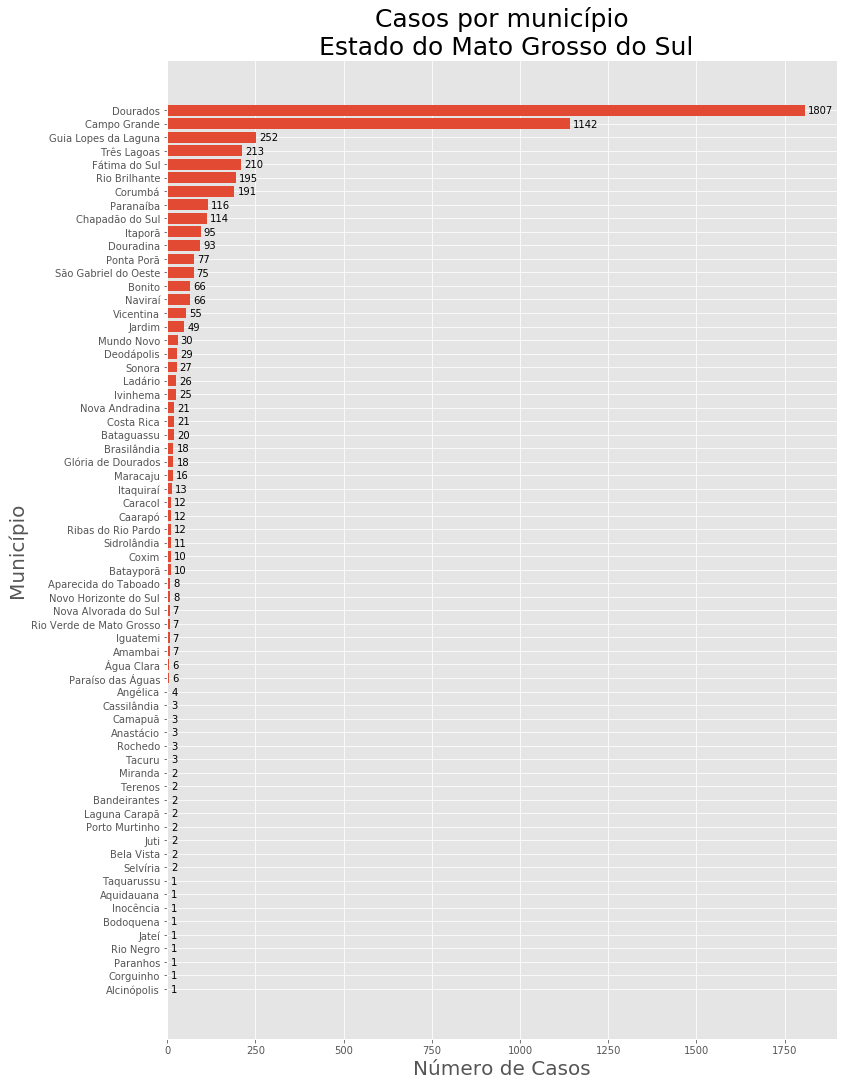
\includegraphics[width=1\textwidth]{figs/casos_por_municipio.png}
  \caption{Número de casos diagnosticados por município (MS)}
  \label{fig:casosMuni}
  \end{figure}

No presente trabalho, uma análise dos dados da cidade de Dourados, MS e apresentada. A situação da cidade é comparada com os demais municípios do estado e a curva de crescimento registrada na referida cidade é comparada com a curva registrada na cidade de Manaus, AM. Em seguida os dados são utilizados para alimentar um modelo preditivo baseado no DELPHI, desenvolvido por uma equipe de pesquisadores ligada ao MIT. Na conclusão, os resultados obtidos são analisados e possíveis desdobramentos de pesquisa sugeridos. 

\section{Metodologia}\label{sec:met}

Mesmo sob a alardeada interiorização da pandemia no Brasil, o caso do município de Dourados, MS chama a atenção pelo fato de, mesmo com uma população equivalente à \(\nicefrac{1}{4}\) da de Campo Grande, apresenta um número total de casos diagnosticados aproximadamente 60\% maior do que os registrados na capital.

A fonte de dados utilizada na elaboração deste relatório foram obtidas no portal \textbf{CORONAVÍRUS BRASIL}\footnote{https://covid.saude.gov.br/}, onde as informações oficiais do Ministério da Saúde sobre a pandemia são disponibilizados. As informações constantes como número de casos (acumulados e novos casos) e sobre a população de cada município foram extraídas desta base. Os dados utilizados foram os disponibilizados do dia 21/06/2020. 

Com base neste conjunto de dados, foram comparados o numero de casos e a população dos diferentes municípios do estado. Representadas em forma de diagramas e mapas (dados geoespaciais) procurando entender como está a distribuição de casos nas diversas regiões do estado. A curva de crescimento dos casos do município foram comparadas com a curva do município de Manaus, AM, procurando entender o quanto esta evolução se aproxima de um caso emblemático da evolução do contágio em território nacional.

\begin{figure}[!htb]
  \centering
  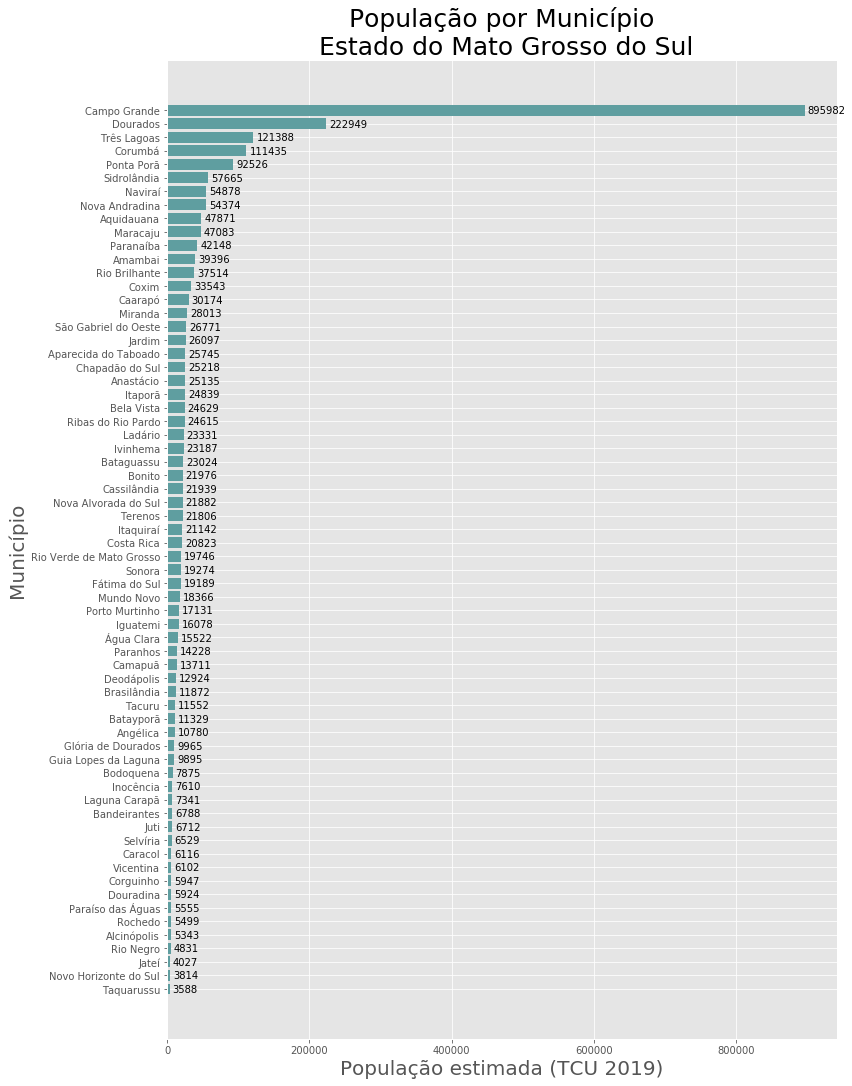
\includegraphics[width=1\textwidth]{figs/pop_por_municipio.png}
  \caption{População por município (MS)}
  \label{fig:popuMuniMS}
  \end{figure}

  Estratégias de visualização de dados e ajuste de polinómios foram utilizadas para ilustrar e entender o caso em estudo. Após essas análises, os dados foram tratados e submetidos ao modelo preditivo escolhido. Ao fim, os resultados são discutidos.

\begin{figure}[!htb]
  \centering
  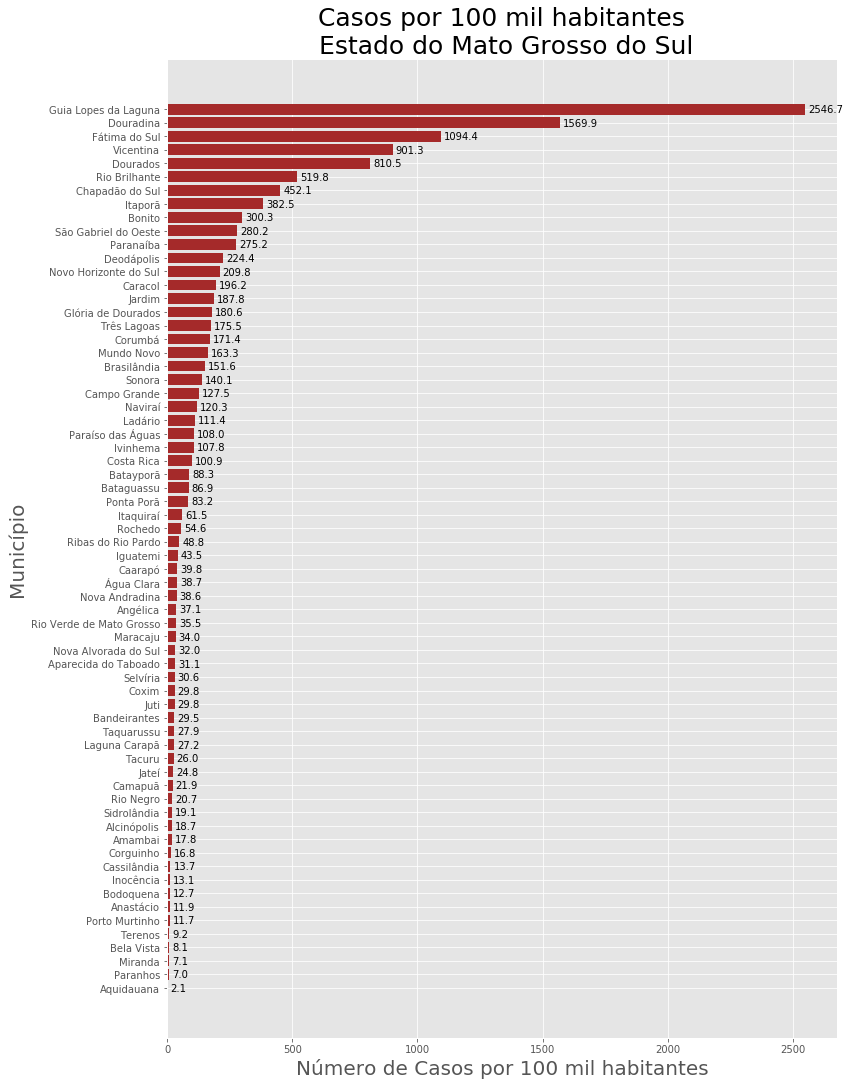
\includegraphics[width=1\textwidth]{figs/casos_100_mil_por_municipio.png}
  \caption{Número de casos por 100 mil habitantes em cada município (MS)}
  \label{fig:casosMuni100k}
  \end{figure}

\section{Análise de Dados}\label{sec:dados}

As figuras~\ref{fig:casosMuni} e~\ref{fig:popuMuniMS} confirmam as informações sobre a  maior incidência de casos em Dourados do que na capital do estado, Campo Grande e mostra que o município está em primeiro lugar em número de casos do estado, sendo a segunda em população do estado.

Já em números relativos, a Figura~\ref{fig:popuMuniMS}, número de casos por 100 mil habitantes, mostra que a cidade objeto deste estudo está em quinto lugar. As cidades que aparecem em sua frente nesta lista, sendo estas: Guia Lopes da Laguna, Douradina, Fátima do Sul e Vicentina, pela ordem, possuem populações muito inferiores. Respectivamente 9895, 5924, 19189 e  6102 habitantes. A de maior população dentre estas (Guia Lopez das Lagunas) apresenta menos de \(\nicefrac{1}{10}\) da população de Dourados. Deve-se levar em conta que, quanto menor a cidade, um mesmo número de casos leva a uma proporção maior quando a análise é ponderada pelo número de habitantes. Ainda assim, estas cidades aparecem em posições altas na lista das maiores em número de casos totais (Fig.~\ref{fig:casosMuni}). Guia Lopes da Laguna, Fátima do Sul, Douradina e Vicentina são respectivamente a terceira(252 casos), quinta(210), décima primeira(93) e décima sexta(93). 

\subsection{Dados Geoespaciais}\label{ssec:geo}

O aspecto geográfico é de grande impacto na análise de dados de um fenômeno com as características de uma epidemia. Os estados, cidades e até mesmo subdivisões menores do espaço como bairros e localidades ou maiores como países e  continentes não delimitam populações estanques e incomunicáveis. As dinâmicas de deslocamento das populações são fundamentais para o entendimento dos caminhos que o vírus percorreu até um determinado local, mas também para estabelecer estratégias de combate eficazes.

\begin{figure}[!htb]
  \centering
  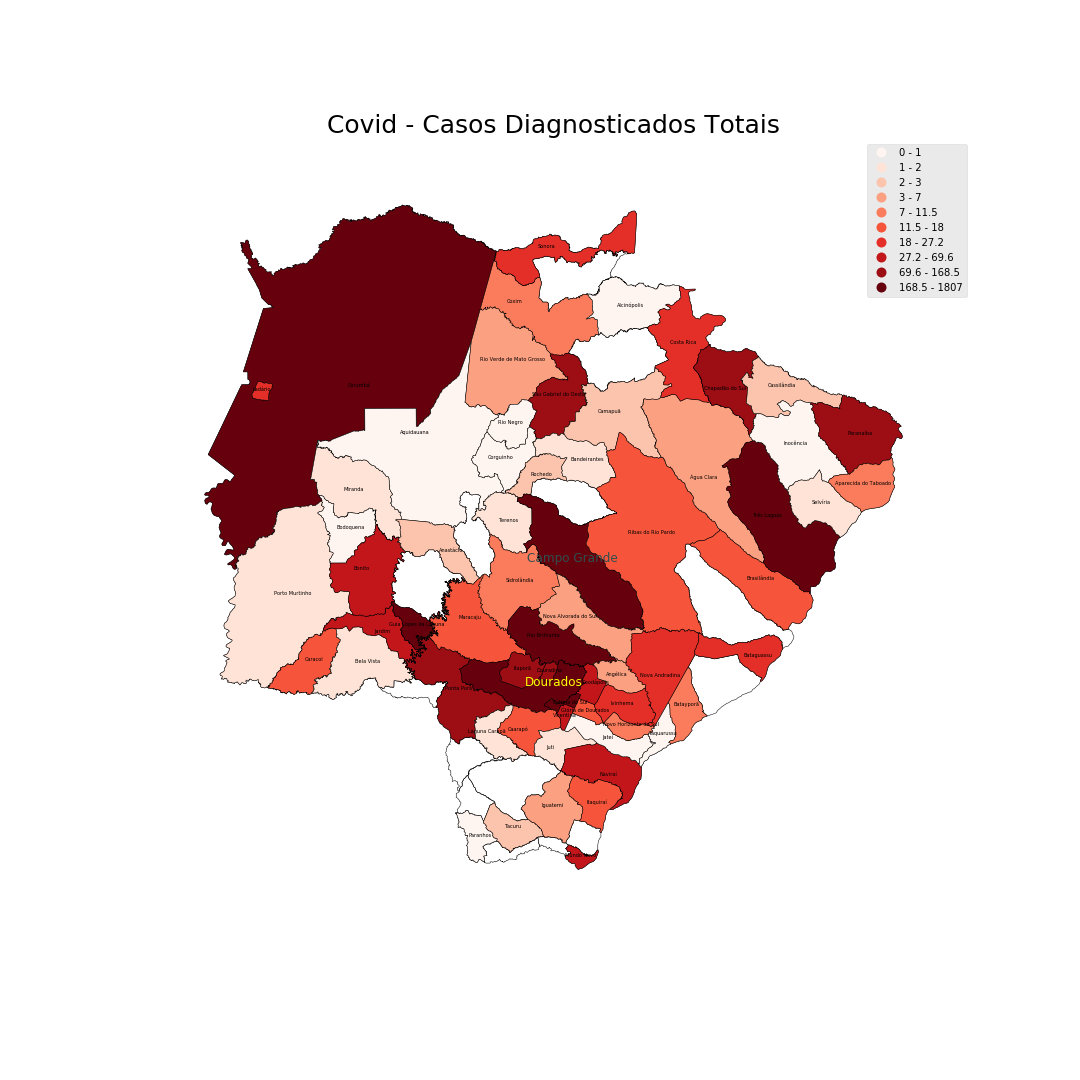
\includegraphics[width=1\textwidth]{figs/mapa_casos_registrados.png}
  \caption{Mapa de casos diagnosticados por município (MS)}
  \label{fig:mapaCasos}
  \end{figure}

Dois mapas foram utilizados para visualizar o cenário atual do estado: Um que mostra os municípios com maior incidência de casos totais (Fig.~\ref{fig:mapaCasos}) e outro que mostra a incidência por cem mil habitantes (Fig.~\ref{fig:mapa100K}). Tanto o município de Dourados, quanto seu entorno aparecem em destaque na escala de cores nos dois mapas.

\begin{figure}[!htb]
    \centering
    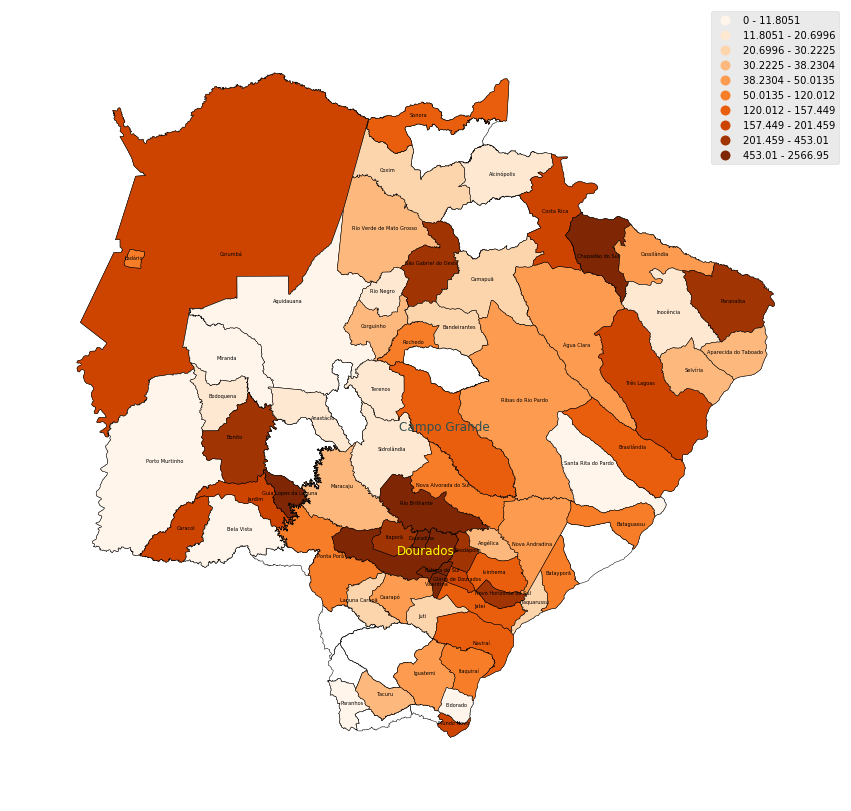
\includegraphics[width=1\textwidth]{figs/mapa_casos_100_mil.png}
    \caption{Número de casos diagnosticados por 100 mil habitantes em cada município (MS)}
    \label{fig:mapa100K}
    \end{figure}
  
Das quatro cidades que apresentam maior número de casos por 100 mil habitantes (Fig.~\ref{fig:casosMuni100k}) apenas Guia Lopes da Laguna não faz fronteira com o município estudado. Considerando as 10 cidades com maior número de casos por 100 mil habitantes seis fazem divisa com o Dourados. Além do próprio estar em quinto lugar da lista temos: Douradina em segundo, Fátima do Sul em terceiro, Vicentina em quarto, Rio Brilhante em sexto Itaporã em oitavo e Deodápolis em décimo. Em primeiro lugar, Guia Lopes da Laguna não está tão distante, fazendo fronteira com dois municípios que possuem divisas com Dourados. 

Em números absolutos Dourados é o primeiro do estado. Totaliza 34\% dos casos confirmados em todo o estado. Considerando os municípios que fazem divisas diretas (Maracaju, Rio Brilhante, Itaporã, Douradina, Deodápolis, Fátima do Sul, Caarapó, Laguna Carapã e Ponta Porã) o obtemos 48\% dos casos registados até a data final deste estudo. Se forem acrescidos os municípios de Vicentina e Glória de Dourados chega-se á praticamente metade (49,7\%) dos casos do estado.

\subsection{Curva de Casos e Comparação com o cenário de Manaus}\label{ssec:curvaMAU}

Os dados apresentados até então apresentam um quadro estático, como um retrato de um momento da pandemia no estado. Para avaliar a evolução do quadro ao longo do tempo, utilizamos a Figura~\ref{fig:curva100K} {fig:curva100KLog} onde pode-se ver os gráficos de casos por 100 mil habitantes a cada dia, e a Figura~\ref{fig:curva100KLog}, que apresenta casos por 100 mil habitantes em escala logarítmica (base 10) por dia. Ambos apresentam a cidade de Dourados comparada a curva de Manaus, AM.

\begin{figure}[!htb]
  \centering
  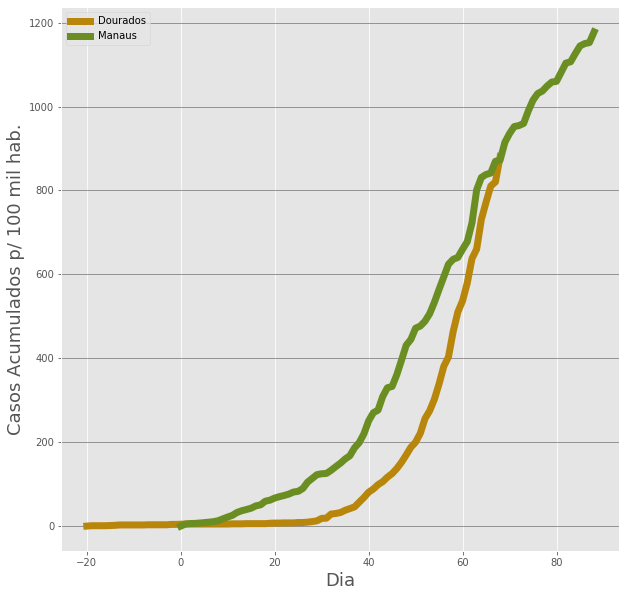
\includegraphics[width=.6\textwidth]{figs/Dourados_Manaus_casos.png}
  \caption{Curva do número de casos diagnosticados por 100 mil habitantes. Comparativo entre Dourados(MS) e Manaus(AM)}
  \label{fig:curva100K}
  \end{figure}

  Na base de dados utilizada o primeiro registro de casos em Manaus e datado no dia 28/03/2020, neste dia são apresentados 105 casos. Considerando a população estimada em 2182763 habitantes da cidade, obtemos uma taxa de 4.81 casos por cem mil habitantes. Já em Dourados, o índice de aproximados 4.81 casos por 100 mil habitantes só é alcançado no dia 14/04/2020.

\begin{figure}[!htb]
  \centering
  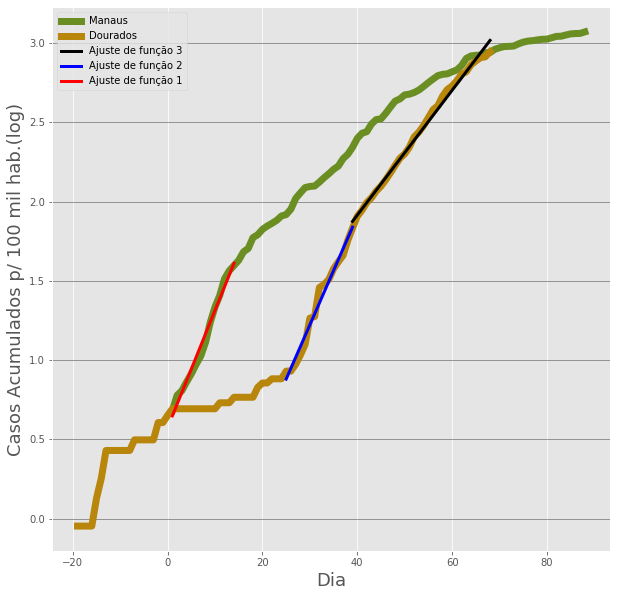
\includegraphics[width=.6\textwidth]{figs/Dourados_Manaus_casos_log.png}
  \caption{Curva do número de casos diagnosticados por 100 mil habitantes. Comparativo entre Dourados(MS) e Manaus(AM) em escala logarítmica (eixo y)}
  \label{fig:curva100KLog}
  \end{figure}

Para efeito de Visualização de dados o dia zero da curva de Dourados foi lançado no mapa na data em que ele alcança a marca inicial do índice de casos por 100 mil habitantes da cidade de Manaus. O Amazonas foi um dos primeiros estados a registrar casos da doença e a evolução até a marca que aparece no primeiro registro não foi registrado, ao menos não pela base de dados utilizada nesta análise. 




\section{Modelo Preditivo}

---

\section{Conclusão}\label{conc}

---

\bibliographystyle{sbc}
\bibliography{sbc-template}

\end{document}
